%% PRESENTATION MODE
\documentclass[
    utf8,
    aspectratio=169
]{beamer}  % We could consider beamerswitch.
%% ARTICLE MODE
%\documentclass[utf8]{article} \usepackage{beamerarticle}

%%% 1. Praeambulum
% Siehe http://www.staff.uni-giessen.de/partosch/unterlagen/Abschlussarbeit-Anleitung.pdf
\usepackage[english]{babel}
\usepackage[%
	backend=biber, %biber would be better, but doesn't work for me so far
	%backend=bibtex8,  %use this backend if biber does not work
	%style=authoryear
	style=numeric,
	maxbibnames=99
	]{biblatex} % Literaturverzeichnis und Zitation
\usepackage{booktabs} % "schoene" Tabellen ermoeglichen
\usepackage[T1]{fontenc} % interne Font-Generierung
\usepackage[hang]{footmisc} % haengende Fussnoten
\usepackage{graphicx} % Abbildungen ermoeglichen
%\usepackage[utf8]{inputenc} % Codierung der Eingabe, set as option in beamer documentclass
\usepackage[scaled]{beramono} % for typewriter family (ttfamily) as used in listings
\usepackage{lmodern} % Schriftfamilie Latin Modern. Als letzten Schrift laden, damit es die aktive ist.
%\usepackage{longtable} % "lange" Tabellen ermoeglichen
%\usepackage{makeidx} % Index ermoeglichen
\usepackage{textcomp} % zusaetzliche LaTeX-Sonderzeichen
 \usepackage{hyperref} % Hypertextstrukturen ermoeglichen, automatically loaded by beamer
%\usepackage{refcheck} % Mit diesem Paket kann man pruefen, ob alle gesetzten Gleichungen auch referenziert werden. Man kann es aber nicht gleichzeitig mit hyperref nutzen.
%\usepackage{xurl} % url mit Umbrücken, am besten nach biblatex laden
\usepackage[babel]{csquotes} % "schoene" Anfuehrungszeichen
\usepackage{xspace}
\usepackage{amsmath}
\usepackage{amssymb}
\usepackage{mathtools}
\usepackage{xfrac}
\usepackage{siunitx}
%\usepackage[most]{tcolorbox}
%\usepackage{etoolbox}
\usepackage{dsfont}
\usepackage{tabularx}
%\usepackage{xparse}
\usepackage{caption}
\usepackage{subcaption}
%\usepackage{amsthm}  % automatically loaded by beamer
%\usepackage{adjustbox}
%\usepackage[boxruled]{algorithm2e}
%\usepackage{xargs}
%%\usepackage{amscd}\usepackage{multirow}
%%\usepackage{lscape}
\usepackage{pgfplots}  % Plots mit tikz/pgf
%\pgfplotsset{compat=1.14}
%\pgfplotsset{compat=1.16}
\pgfplotsset{compat=1.18}
%\usepackage{tikz} % draw graphics, diagrams and boxes
%\usetikzlibrary{arrows.meta, calc, decorations.text, decorations.pathmorphing, positioning, shapes.misc}
% overlay-beamer-styles is from package aobs-tikz
\usetikzlibrary{calc, positioning, shapes.geometric, tikzmark, decorations.pathreplacing, calligraphy, overlay-beamer-styles}
\usepackage{listings} % verbatim and code style
\usepackage{fontawesome5}
%\usepackage{awesomebox} % nice message boxes
%\usepackage[]{draftwatermark}
%\SetWatermarkColor[gray]{0.9}
\usepackage{placeins}  % \FloatBarrier
%\usepackage[section]{placeins}  % force floating figures before new section
\usepackage{exercise}

% bib-file for bibliography
\addbibresource{lecture_slides_Bib.bib}

% Wir wollen Grossbuchstaben für Chapter, Section and Subsection,
% so wie es für Figure, Table, etc. bereits der Default ist.
% Siehe Dokumentation for hyperref.
\addto\extrasenglish{
    \def\chapterautorefname{Chapter}
	\def\sectionautorefname{Section}
	\def\subsectionautorefname{Subsection}
	\def\subsubsectionautorefname{Subsubsection}
	\def\paragraphnameautorefname{Paragraph}
}


% Modifikationen am Textsatz und Layout
% \emph innerhalb einer definition Environment bold statt italic
% siehe https://tex.stackexchange.com/questions/315058/change-the-behaviour-of-emph-per-environment/330491
\AtBeginEnvironment{definition}{\renewcommand\eminnershape{\bfseries}}

% If beramono is imported after lmodern, we might want to change some use cases of typewriter back to latin modern type writer.
% We revert this for some use cases like url links:
%\renewcommand\UrlFont{\color{cyan}\fontfamily{lmtt}\selectfont} % lmtt is latin modern typewriter

\newcommand{\pkg}[1]{{\normalfont\fontseries{b}\selectfont #1}}
\let\proglang=\textsf
\let\code=\texttt
\let\variable=\texttt

%listings
% We want to avoid that in "my_log_constant", "log" is highlighted, and therefore remove _ from otherkeywords and from alsoother, see
% https://tex.stackexchange.com/questions/318841/listings-with-r-keywords-in-variable-names-are-highlighted-when-using-underscor
\lstset{
	%basicstyle=\scriptsize\ttfamily,
	basicstyle=\fontfamily{fvm}\selectfont\scriptsize, % fvm is beramono, see file beramono.sty
	columns=fixed,
	numbers=none, %left,
	%escapeinside=||,
	breakatwhitespace=true,
	language=R,
	otherkeywords={!,!=,~,$,*,\&,\%/\%,\%*\%,\%\%,<-,<<-,/},
	alsoother={.$},
	%deletekeywords={_},
	frame=tb,
	tabsize=4 %default is 8
}
%%Modify caption type for algorithms2e
%\makeatletter
%\renewcommand{\@algocf@capt@plain}{above}% formerly {bottom}
%\makeatother
% eigene Vereinbarung:
\newcommand*{\eg}{e.g.,\@\xspace}
\newcommand*{\ie}{i.e.\@\xspace}
\newcommand*{\cf}{cf.\@\xspace}
\newcommand*{\etc}{etc.\@\xspace}
\newcommand*{\wrt}{w.r.t.\@\xspace}
\newcommand*{\iid}{i.i.d.\@\xspace}
\DeclareMathOperator{\Prob}{\mathbb{P}}
\DeclareMathOperator{\E}{\mathbb{E}}  % alternative: \mathbf{E}
\newcommand{\eps}{\varepsilon}
\newcommand{\R}{\mathbb{R}}
\renewcommand{\P}{\mathbb P}
\newcommand{\M}{\mathcal M}
\newcommand{\X}{\mathcal X}
\newcommand{\Y}{\mathcal Y}
\newcommand{\bx}{\boldsymbol{x}}
\newcommand{\bX}{\boldsymbol{X}}
\def\realnumbers{\mathbb{R}}

% Color in math environments
% https://tex.stackexchange.com/a/261480
\makeatletter
\def\mathcolor#1#{\@mathcolor{#1}}
\def\@mathcolor#1#2#3{%
  \protect\leavevmode
  \begingroup
    \color#1{#2}#3%
  \endgroup
}
\makeatother


% Beamer Stuff
\usetheme{default}
\useinnertheme{default}
\useoutertheme{default}
\setbeamertemplate{navigation symbols}{}  % no navigation at all
% https://tex.stackexchange.com/a/137028
\addtobeamertemplate{navigation symbols}{}{%
    \usebeamerfont{footline}%
    \usebeamercolor[fg]{footline}%
    \hspace{1em}%
    \insertframenumber/\inserttotalframenumber
}

% https://getbootstrap.com/docs/5.0/customize/color/
% Bootstrap Color Palette
% blue: #0d6efd
% indigo: #6610f2
% purple: #6f42c1 
% pink: #d63384 
% red: #dc3545
% orange: #fd7e14
% yellow: #ffc107
% green: #198754
% teal: #20c997
% cyan: #0dcaf0 
% gray-500: #adb5bd
\definecolor{BCPblue}{HTML}{0d6efd}
\definecolor{BCPgreen}{HTML}{198754}
\definecolor{BCPred}{HTML}{dc3545}

%\setbeamercolor{section in toc}{fg=black,bg=white}
%\setbeamercolor*{palette primary}{fg=darkred!60!black,bg=gray!30!white}
%\setbeamercolor*{palette secondary}{fg=darkred!70!black,bg=gray!15!white}
%\setbeamercolor*{palette tertiary}{bg=darkred!80!black,fg=gray!10!white}
%\setbeamercolor*{palette quaternary}{fg=darkred,bg=gray!5!white}
\setbeamercolor{structure}{fg=BCPblue} % itemize, enumerate, etc
\setbeamercolor{example text}{fg=BCPgreen}
\setbeamercolor{alerted text}{fg=BCPred}

%\setbeamercolor*{sidebar}{fg=darkred,bg=gray!15!white}

%\setbeamercolor*{palette sidebar primary}{fg=darkred!10!black}
%\setbeamercolor*{palette sidebar secondary}{fg=white}
%\setbeamercolor*{palette sidebar tertiary}{fg=darkred!50!black}
%\setbeamercolor*{palette sidebar quaternary}{fg=gray!10!white}

%%\setbeamercolor*{titlelike}{parent=palette primary}
%\setbeamercolor{titlelike}{parent=palette primary,fg=darkred}
%\setbeamercolor{frametitle}{bg=gray!10!white}
%\setbeamercolor{frametitle right}{bg=gray!60!white}

%\setbeamercolor*{separation line}{}
%\setbeamercolor*{fine separation line}{}

% ToC before each section
\AtBeginSection[]
{
  \begin{frame}
    \frametitle{Table of Contents}
    \tableofcontents[currentsection]
  \end{frame}
}

\titlegraphic{
    
\includegraphics[width=3cm]{logo.png}
}

%%% 2. Documentum

\title{Introduction to Machine Learning}
\author{Michael Mayer}
%\institute{}
\date{October 2022}

%=====================================================================
\begin{document}
%=====================================================================

\frame{\titlepage}

% \setcounter{tocdepth}{1}
% \begin{frame}
%     \frametitle{Table of Contents}
%     \tableofcontents
% \end{frame}
% \setcounter{tocdepth}{2}

%=====================================================================
\section{Intro}
%=====================================================================

\begin{frame}
\begin{quotation}
	\begin{huge}
		\begin{center}
			Data Science is 90\% data preparation.
	
			This lecture is about the remaining 10\%.
		\end{center}
	\end{huge}
\end{quotation}
\end{frame}

\begin{frame}
	\frametitle{About Michael}
	\begin{itemize}
		\item Pricing actuary at Swiss Mobiliar
		\item Lecturer at ETH Zurich
		\item PhD in statistics
		\item $(M+C)^2$ Blog: \url{https://lorentzen.ch/}
		\item \url{https://github.com/mayer79}
	\end{itemize}
\end{frame}

\begin{frame}
	\frametitle{What is Machine Learning (ML)?}
	\begin{columns}
		\column{0.55\textwidth}
		\begin{block}{Collection of statistical algorithms used to}
			\begin{enumerate}
				\item predict things (supervised ML) or to
				\item investigate data structure 
				
				(unsupervised ML).
			\end{enumerate}
		\end{block}	
		\begin{block}{This lecture is on supervised ML}
			\begin{itemize}
				\item Regression
				\item Classification
			\end{itemize}
		\end{block}
		\column{0.4\textwidth}
		\begin{figure}
			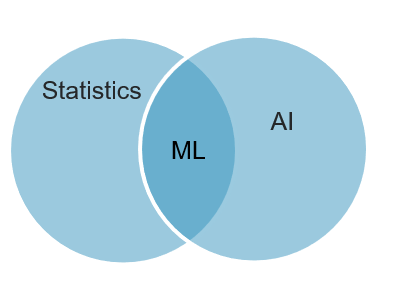
\includegraphics[width=0.95\textwidth]{pics/ml.png}
		\end{figure}
	\end{columns}
\end{frame}

\begin{frame}
	\frametitle{Lecture Overview}
	\begin{block}{Chapters}
		\begin{enumerate}
			\item Basics and Linear Models
			\item Model Selection and Validation
			\item Trees
			\item Neural Nets
		\end{enumerate}
	\end{block}
	
	\begin{block}{Material}
		\url{https://github.com/mayer79/ml\_lecture}
	\end{block}
\end{frame}

%=====================================================================
\section{Basics and Linear Models}
%=====================================================================

%=====================================================================
\subsection{Basics}
%=====================================================================

\begin{frame}
	\frametitle{Before Modeling}
	\begin{columns}
		\column{0.35\textwidth}
		\begin{itemize}
			\item Organization of data?
			\item Data types?
			\item Descriptive analysis
		\end{itemize}
		\begin{figure}
			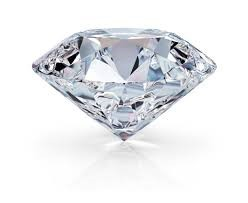
\includegraphics[width=0.6\textwidth]{pics/diamond.jpg}
		\end{figure}
		\column{0.65\textwidth}
		\begin{block}{\centering Structure of diamonds data}
		\begin{table}
			\begin{tabular}{ccccc}
				\hline
				price &carat &color &cut  & clarity \\
				\hline
				326&  0.23& E&     Ideal&     SI2   \\ 
				326&  0.21& E&     Premium&   SI1   \\ 
				327&  0.23& E&     Good  &    VS1   \\ 
				334&  0.29& I&     Premium&   VS2   \\ 
				335&  0.31& J&     Good  &    SI2   \\ 
				336&  0.24& J&     Very Good &VVS2 \\
				\hline
			\end{tabular}
		\end{table}
		\end{block}
	
		\begin{example}
		\end{example}
	\end{columns}
\end{frame}

\begin{frame}
	\frametitle{Statistical Models}
	\begin{block}{Setting}
		\begin{itemize}
			\item Approximate \alert{response variable} $Y$ by function $f$ of \alert{covariates} $X_1,\dots,X_m$
			$$
				Y \approx f(X_1,\dots,X_m)
			$$
			\item Estimate unknown $f$ from data by $\hat f$.
			\item Use $\hat f$ for prediction and to investigate relationships.
			\item Postulate model equation $\E(Y) = f(X_1, \dots, X_m)$
			
			(we are often interested in means).
		\end{itemize}
	\end{block}
	
	\begin{block}{Remark}
		Other terms for response and covariates?
	\end{block}
\end{frame}

%=====================================================================
\subsection{Linear Regression}
%=====================================================================

\begin{frame}
	\frametitle{Linear Regression}
	\begin{itemize}
		\item Postulate 
		$$
			\E(Y) = f(X_1, \dots, X_m)=\beta_0 + \beta_1 X_1 + \dots + \beta_m X_m
		$$
		\item Interpretation of coefficients $\beta_j$? Ceteris Paribus!
		\item Optimal $\hat \beta_j$? Minimize sum of squared errors/residuals
		$$
			\sum_{i = 1}^n (\underbrace{y_i - \hat y_i}_{\text{\alert{Residual}}})^2 
		$$
		\item $\hat y = \hat f(\dots)$ are \alert{predictions}
	\end{itemize}

	\vfill
	
	\begin{example}
		Simple linear regression: $\E(Y)=\alpha = \beta X$
	\end{example}
\end{frame}

\begin{frame}
	\frametitle{Aspects of Model Quality}
	\begin{columns}[onlytextwidth]
		\column{0.5\textwidth}
		\begin{block}{Predictive performance}
			\begin{itemize}
				\item Absolute performance
					\begin{itemize}
						\item $\text{\alert{MSE}} = \frac{1}{n}\sum_{i = 1}^n (y_i - \hat y_i)^2$
						\item Root-MSE (\alert{RMSE})
						\item Loss and objective functions	
					\end{itemize}
				\item Relative performance
					\begin{itemize}
						\item \alert{R-squared}
					\end{itemize}
			\end{itemize}
		\end{block}	
	
		\column{0.5\textwidth}
		\begin{block}{Validity of assumptions}
			\begin{itemize}
				\item Model equation is correct
				\item \alert{Normal} linear model
				 \begin{align*}
					 Y &= f(\dots) + \varepsilon \\
					 \varepsilon &\sim N(0, \sigma^2)
				 \end{align*}
			\end{itemize}
		\end{block}
	\end{columns}

	\vfill
	
	\begin{exampleblock}{\centering Example}
	\end{exampleblock}
\end{frame}

\begin{frame}
	\frametitle{Typical Problems}
	\begin{figure}
		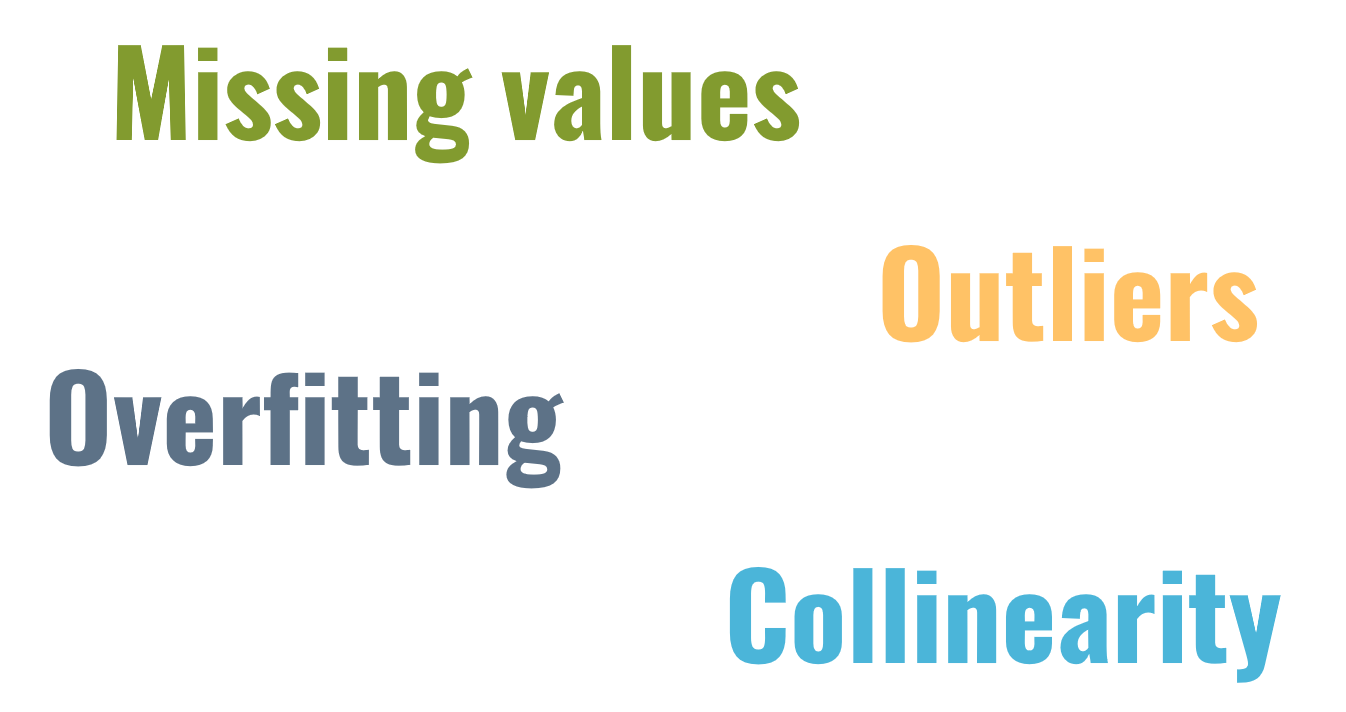
\includegraphics[width=0.7\textwidth]{pics/linear_problems.png}
	\end{figure}
\end{frame}

\begin{frame}
	\frametitle{Categorical Covariates}
	\begin{columns}[onlytextwidth]
		\column{0.45\textwidth}
		\begin{itemize}
			\item One-Hot-Encoding
			\item Dummy coding
			\item Interpretation?
		\end{itemize}
	
		\vspace{1cm}
	
		\begin{example}
		\end{example}
	
		\column{0.45\textwidth}
		\begin{block}{\centering Example of One-Hot-Encoding}
			\begin{small}
				\begin{table}
					\begin{tabular}{c|ccccccc}
						   color& D& E& F &G&H &I &J \\
				  		\hline
						E  &   0  &   1  &   0  &   0  &   0  &   0  &   0 \\
						E  &   0  &   1  &   0  &   0  &   0  &   0  &   0 \\
						E  &   0  &   1  &   0  &   0  &   0  &   0  &   0 \\
						I  &   0  &   0  &   0  &   0  &   0  &   1  &   0 \\
						J  &   0  &   0  &   0  &   0  &   0  &   0  &   1 \\
						J  &   0  &   0  &   0  &   0  &   0  &   0  &   1 \\
						I  &   0  &   0  &   0  &   0  &   0  &   1  &   0 \\
						H  &   0  &   0  &   0  &   0  &   1  &   0  &   0 \\
						E  &   0  &   1  &   0  &   0  &   0  &   0  &   0 \\
						H  &   0  &   0  &   0  &   0  &   1  &   0  &   0 \\
				     	\hline
					\end{tabular}
				\end{table}
			\end{small}
		\end{block}
	\end{columns}
\end{frame}

\begin{frame}
	\frametitle{Linear Regression is Flexible}
	\begin{enumerate}
		\item Non-linear terms
		\item Interactions
		\item Transformations like logarithms
	\end{enumerate}
	
	\vfill
	
	\begin{alertblock}{These elements are essential but tricky!}
	\end{alertblock}
\end{frame}

\begin{frame}
	\frametitle{Non-Linear Terms}
	\begin{columns}
		\column{0.5\textwidth}
		\begin{block}{Deal with non-linear associations to $Y$?} $\rightarrow$ invest more parameters
		\begin{enumerate}
			\item Polynomial terms
			\begin{itemize}
				\item E.g., cubic regression
				$$
					\E(Y) = \beta_0 + \beta_1 x + \beta_2 x^2 + \beta_3 x^3
				$$
				\item Don't extrapolate!
			\end{itemize}
			\item Regression splines
		\end{enumerate}
		\end{block}
		
		\column{0.5\textwidth}
		\begin{block}{\centering Cubic terms for carat}
			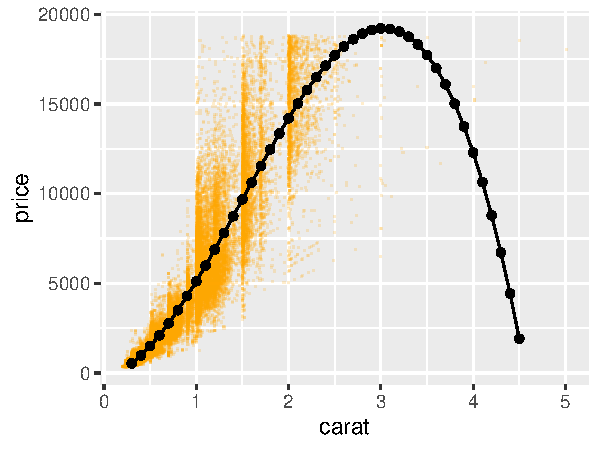
\includegraphics[width=1\textwidth]{pics/nonlinear.pdf}
			\vspace{-9em}
			\begin{scriptsize}
				\begin{table}
					\raggedleft
					\begin{tabular}{ccc}
						carat & carat$^2$ & carat$^3$ \\
								\hline
						 0.23       &            0.0529       &          0.012167\\
						 0.21       &            0.0441       &          0.009261\\
						 0.23       &            0.0529       &          0.012167\\
					\hline
					\end{tabular}
				\end{table}
			\end{scriptsize}
			\vspace{3em}
			\centering Use systematic predictions
		\end{block}
	\end{columns}
\end{frame}

\begin{frame}
	\frametitle{Interactions}
	\begin{columns}
		\column{0.55\textwidth}
		\begin{itemize}
			\item Additivity of effects not always realistic
			$$
				\E(Y) = \beta + \beta_1 X_1 + \dots + \beta_m X_m
			$$
			\item Adding interaction terms brings necessary flexibility 
			$\rightarrow$ more parameters
			\item Interaction between features $X$ and $Z$
			\begin{itemize}
				\item For categorical $Z$, effects of $X$ are calculated by level of $Z$
				\item Like separate models per level of $Z$
			\end{itemize}
		\end{itemize}
		
		\column{0.45\textwidth}
		\begin{block}{\centering Carat and color}
			\begin{figure}
				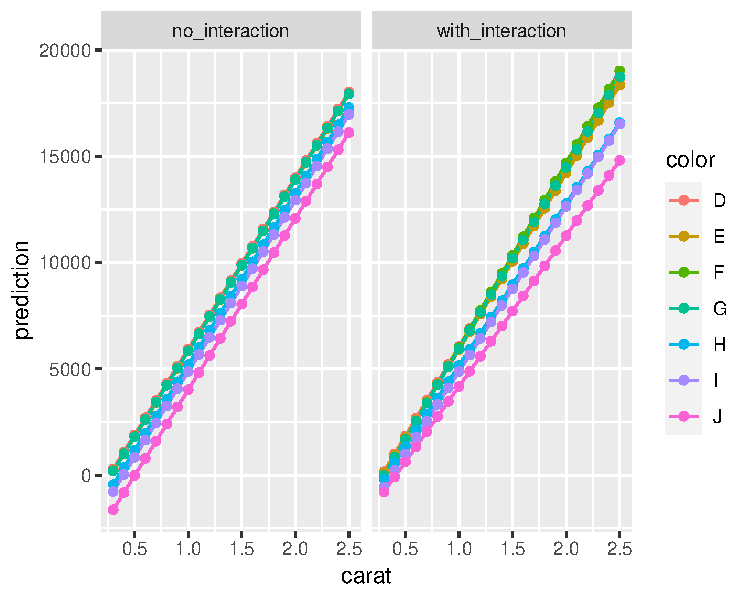
\includegraphics[width=\textwidth]{pics/interaction.pdf}
			\end{figure}
		\end{block}
	\end{columns}
\end{frame}

\begin{frame}
	\frametitle{Transformations of Covariates}
	\begin{block}{Examples}
		\begin{itemize}
			\item Dummy variables for categoricals
			\item Decorrelation
			\item Logarithms against outliers
		\end{itemize}
	\end{block}
	
	\vfill
	
	Effects are interpreted for transformed covariates
\end{frame}

\begin{frame}
	\frametitle{Logarithmic Covariates}
	\begin{itemize}
		\item $\E(Y) = \alpha + \beta\log(X)$
		\item Properties of logarithm allow interpretation \alert{for original covariate}
		\item ``A 1\% increase in $X$ leads to an increase in $\E(Y)$ of about $\beta/100$''
		
		($\rightarrow$ lecture notes)
		
		\vfill
		
		\begin{example}
		\end{example}
	\end{itemize}
\end{frame}

\begin{frame}
	\frametitle{Logarithmic Responses}
	What would happen for logarithmic response?
	\begin{align*}
		\E(\log(Y)) &= \alpha + \beta X \\
		\implies \log(\E(Y)) &= \alpha + \beta X?
	\end{align*}
	The implication is wrong (why?) $\rightarrow$ biased predictions and motivation for GLMs
	
	\begin{itemize}
		\item ``A one-point increase in $X$ is associated with a relative increase in $\E(Y)$ of $100\%(e^\beta - 1)\approx 100\% \beta$''
		$\rightarrow$ lecture notes
		\item Relative effects / multiplicative model
	\end{itemize}
	
	\begin{exampleblock}{Examples}
		\begin{itemize}
			\item Logarithmic response
			\item Response and covariate with log
		\end{itemize}
	\end{exampleblock}
\end{frame}

\begin{frame}
	\frametitle{Example: Realistic Model for Diamond Prices}
	\begin{columns}
		\column{0.55\textwidth}
		\begin{itemize}
			\item Response: log(price)
			\item Covariates: log(carat), color, cut and clarity
		\end{itemize}
	
		\column{0.35\textwidth}
		\begin{figure}
			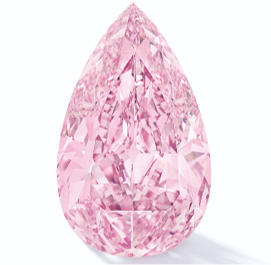
\includegraphics[width=0.7\textwidth]{pics/dia2.png}
		\end{figure}
	\end{columns}
\end{frame}

\begin{frame}
	\frametitle{Exercise on Linear Regression}
	\begin{columns}
		\column{0.55\textwidth}
		\begin{itemize}
			\item Run last model without any logarithm
			\item Interpret the results
			\item Does model make sense from practical perspective?
		\end{itemize}
		\column{0.35\textwidth}
		\begin{figure}
			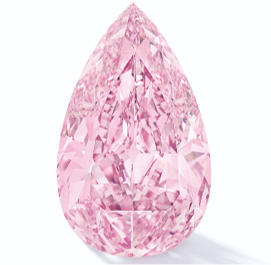
\includegraphics[width=0.7\textwidth]{pics/dia2.png}
		\end{figure}
	\end{columns}
\end{frame}

%=====================================================================
\subsection{Generalized Linear Models}
%=====================================================================

\begin{frame}
	\frametitle{Generalized Linear Model (GLM)}
	\begin{block}{(One) extension of linear regression}
	\end{block}
	
	\begin{block}{Model equation}
		Two equivalent formulations
		\begin{align*}
			g(\E(Y)) &= \beta_0 + \beta_1 X_1 + \dots + \beta_m X_m \\
			\E(Y) &= g^{-1}(\beta_0 + \beta_1 X_1 + \dots + \beta_m X_m)
		\end{align*}
	\end{block}
	
	\begin{block}{Components}
		\begin{itemize}
			\item Linear function/predictor
			\item Link function $g$ to map $\E(Y)$ to linear scale
			\item Distribution of $Y$ conditional on covariates
		\end{itemize}
	\end{block}
\end{frame}

\begin{frame}
	\frametitle{Typical GLMs}
	\begin{columns}[onlytextwidth]
		\column{0.75\textwidth}
		\begin{footnotesize}
			\begin{figure}
				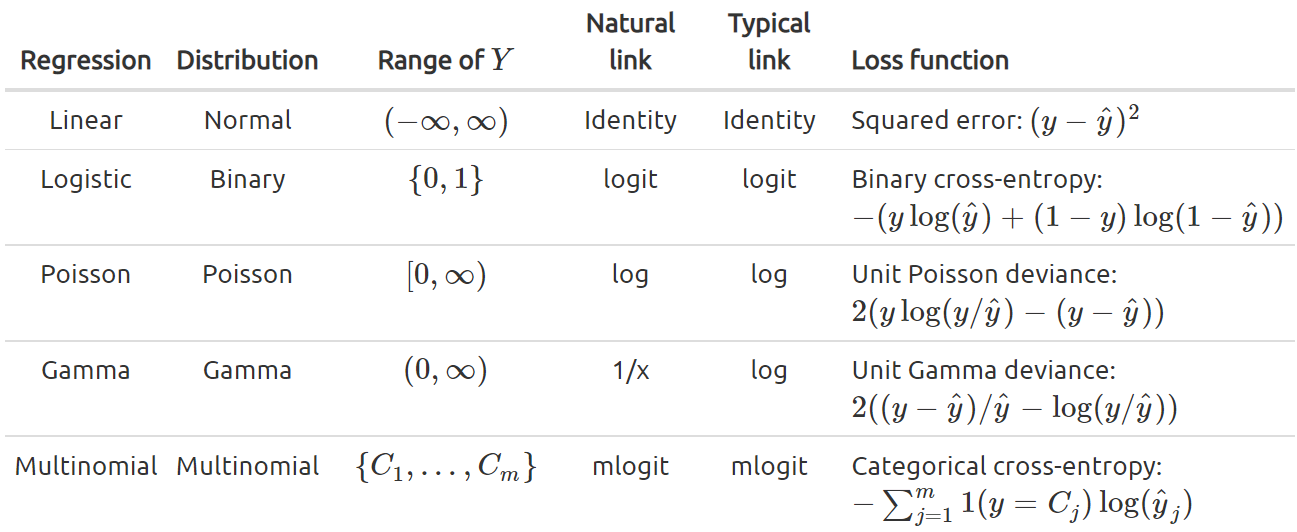
\includegraphics[width=1\textwidth]{pics/glm.png}
			\end{figure}
		\end{footnotesize}
		\column{0.25\textwidth}
		\begin{footnotesize}
			\begin{itemize}
				\itemsep0em 
				\item Predictions?
				\item Log-Link?
				\item For binary $Y$:
				$\E(Y) = P(Y = 1) = p$
				\item Tweedie-GLM
				\item MSE $\rightarrow$ Deviance
				\item Same losses for ML
			\end{itemize}
		\end{footnotesize}
	\end{columns}

	\begin{figure}
		\includegraphics[width=0.8\textwidth]{pics/GLM_distributions.pdf}
	\end{figure}
\end{frame}

\begin{frame}
	\frametitle{Why GLM, not Linear Regression?}
	\begin{block}{Linearity assumption not always realistic}
		\begin{enumerate}
			\item Binary $Y$: 
			
			Jump from 0.5 to 0.6 success probability less impressive than from 0.89 to 0.99
			\item Count $Y$: Jump from $\E(Y)$ of 2 to 3 less impressive than from 0.1 to 1.1.
			\item Right-skewed $Y$: 
			
			Jump from 1 Mio to 1.1 Mio deemed larger than from 2 Mio to 2.1 Mio.
		\end{enumerate}
	\alert{Logarithmic $Y$ not possible in the first two cases}
	\end{block}

	\vfill
	
	\begin{block}{GLM solves problem by suitable link $g$}
	\end{block}
	
	\vfill
	
	\begin{block}{Further advantages?}
	\end{block}
\end{frame}

\begin{frame}
	\frametitle{Interpretation of Effects guided by Link}
	\begin{columns}[onlytextwidth]
		\column{0.5\textwidth}
		\begin{block}{Identity link}
			Like linear regression
		\end{block}
		
		\begin{block}{Log link}
			Like linear regression with log response
			\begin{itemize}
				\item Multiplicative model for response
				\item Now in mathematically sound way
			\end{itemize}
		\end{block}
		
		\column{0.5\textwidth}
		\begin{block}{Logit link}
			\begin{itemize}
				\item Additive model for $\text{logit}(p)$
				\item $\text{logit}(p) = \text{\alert{log}}(\text{odds}(p)) = \text{\alert{log}}\left(\frac{p}{1-p}\right)$
				\item Remember: $p = P(Y=1) = \E(Y)$				
				\item Multiplicative model for $\text{odds}(p)$
				\item Coefficients \alert{$e^\beta - 1 \approx 100\%\beta$} interpreted as odds ratios
			\end{itemize}
		\end{block}
	\end{columns}
\end{frame}

\begin{frame}
	\frametitle{Examples with Insurance Claim Data}
	\begin{enumerate}
		\item Poisson regression for claim counts
		\item Binary logistic regression for claim (yes/no)
	\end{enumerate}
\end{frame}

\begin{frame}
	\frametitle{Exercise on GLM}
	\begin{columns}
		\column{0.55\textwidth}
		\begin{itemize}
			\item Fit Gamma regression with log-link to explain diamond prices by log(carat), color, cut and clarity. 
			\item Compare the coefficients with corresponding linear regression for log(price).
			\item Evaluate the relative prediction bias on USD scale.
		\end{itemize}
		\column{0.35\textwidth}
		\begin{figure}
			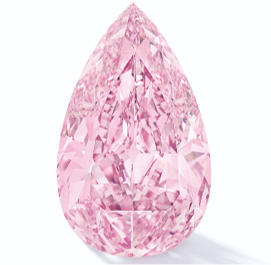
\includegraphics[width=0.7\textwidth]{pics/dia2.png}
		\end{figure}
	\end{columns}
\end{frame}

%=====================================================================
\section{Model Selection and Validation}
%=====================================================================

\begin{frame}
	\frametitle{Two Questions}
	
	\begin{itemize}
		\item ``How good is our model?''
		\item ``Which model to choose among alternatives?''
	\end{itemize}
	
	\vfill
	
	\begin{columns}[onlytextwidth]
		\column{0.5\textwidth}
		\begin{block}{Problem and solution}
			\begin{itemize}
				\item ``Insample'' performance is biased
				\item Overfitting should not be rewarded
				\item Use data splitting to get fair results
			\end{itemize}
		\end{block}
	
		\column{0.5\textwidth}
		\begin{alertblock}{Remarks}
			\begin{itemize}
				\item Performance measure (evaluation metric) versus loss function?
				\item Confusion matrix?
			\end{itemize}
		\end{alertblock}
	\end{columns}
\end{frame}

\begin{frame}
	\frametitle{Excursion: $k$-Nearest-Neighbour ($k$-NN)}
	\begin{itemize}
		\item Alternative to linear model
		\item How does it work?
		\item Classification and Regression
		\item Standardization?
	\end{itemize}
	
	\vfill
	
	\begin{example}
	\end{example}
\end{frame}

\begin{frame}
	\frametitle{Simple Validation}
	\begin{itemize}
		\item Insample, 1-NN would win any comparison!?
		\item Split data into training and validation set, e.g., 80\%/20\%
		\item Use performance on validation set to make decisions 
		
		(choose models, choose parameters like $k$)
		\item Measure amount of overfitting (= optimism)?
	\end{itemize}

	\vfill
	
	\begin{example}
	\end{example}
\end{frame}

\begin{frame}
	\frametitle{Cross-Validation (CV)}
	
	Simple validation is neither economic nor robust, except for large data
	
	\vfill
	
	\begin{columns}[onlytextwidth]
		\column{0.65\textwidth}
		\begin{block}{Algorithm}
			\begin{enumerate}
				\item Split the data into $k$ pieces $D = \{D_1, \dots, D_k\}$ called ``folds''. Typical $k$?
				\item Set aside one of the pieces ($D_j$) for validation.
				\item Fit model on all other pieces, i.e., on $D \setminus D_j$.
				\item Calculate performance on the validation data $D_j$.
				\item Repeat Steps 2--4 until each piece was used for validation once.
				\item The average of the $k$ model performances yields the \alert{CV performance} of the model.
			\end{enumerate}
		\end{block}
		
		\column{0.35\textwidth}
		\begin{alertblock}{Remarks}
			\begin{itemize}
				\item How to choose and fit best/final model? 
				\item What means «best»?
				\item Repeated CV?
			\end{itemize}
		\end{alertblock}
	
		\begin{example}
		\end{example}
	\end{columns}
\end{frame}

\begin{frame}
	\frametitle{Hyperparameter Tuning}
	\begin{itemize}
		\item Choosing $k$ in $k$-NN is example of \alert{``hyperparameter tuning''}
		\item Algorithms with more than 1 hyperparameter?
		\item Grid Search CV
		\item Randomized Search CV
	\end{itemize}
\end{frame}

\begin{frame}
	\frametitle{Test Data and Final Workflow}
	
	\begin{block}{Problematic consequence of model tuning?}
		\begin{itemize}
			\item \alert{Overfitting} on validation data or on CV!
			\item Performance of final model? $\rightarrow$ \alert{Test data}
		\end{itemize}
	\end{block}
	
	\begin{columns}[onlytextwidth]
		\column{0.55\textwidth}
		\begin{block}{Workflow A}
			\begin{footnotesize}
				\begin{enumerate}
					\item Split data into train/valid/test, 
					
					e.g., by ratios 70\%/20\%/10\%.
					\item Train different models on training data and assess their performance on the validation data. Choose best model, retrain on combination of training and validation data and call it ``final model''.
					\item Assess performance of final model on test data.
				\end{enumerate}
			\end{footnotesize}
		\end{block}
		
		\column{0.45\textwidth}
		\begin{block}{Workflow B}
			\begin{footnotesize}
				\begin{enumerate}
					\item Split data into train/test, 
					
					e.g., by ratios 90\%/10\%.
					\item Evaluate and tune different models by $k$-fold CV on the training data. Choose best model, retrain on full training data.
					\item Assess performance of final model on test data.
				\end{enumerate}
			\end{footnotesize}
		\end{block}
	\end{columns}

	\begin{columns}
		\column{0.5\textwidth}
		\begin{exampleblock}{Example of Workflow B}
		\end{exampleblock}
	
		\column{0.5\textwidth}
		\alert{When Test = Validation?}
	\end{columns}
\end{frame}

\begin{frame}
	\frametitle{Using Independent Partitions is Essential}
	\begin{figure}
		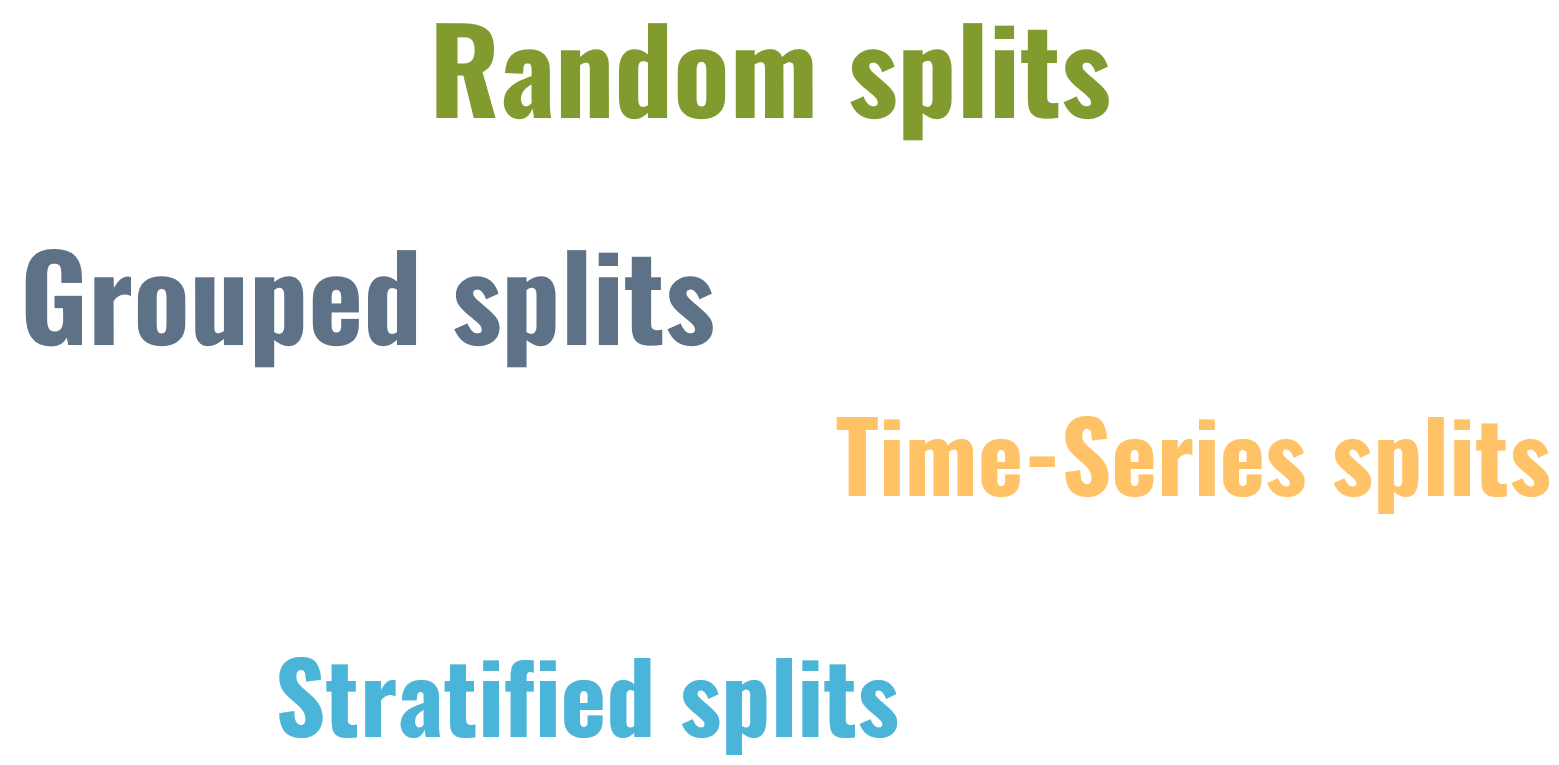
\includegraphics[width=0.8\textwidth]{pics/validation_independent.png}
	\end{figure}
\end{frame}

\begin{frame}
	\frametitle{Exercises with Diamonds}
	\begin{enumerate}
		\item As alternative to grouped splitting, deduplicate (why?) the diamonds data on "price" and all covariates and repeat the last example. Do the results change? Which results do you trust more?
		
		\vfill
		
		\item Use CV to select the best polynomial degree of log(carat) in the Gamma GLM with log-link (with additional covariates color, cut, clarity). Evaluate on a test data.
	\end{enumerate}
\end{frame}

%=====================================================================
\section{Trees}
%=====================================================================

%=====================================================================
\subsection{Decision Trees}
%=====================================================================

\begin{frame}
	\frametitle{Trees}
	\begin{figure}
		
\includegraphics[width=0.7\textwidth]{pics/tree_outline.png}
	\end{figure}
\end{frame}

\begin{frame}
	\frametitle{Decision Trees}
	\begin{columns}[onlytextwidth]
		\column{0.5\textwidth}
		\begin{itemize}
			\item Simple		
			\item Easy to interpret
			\item Decision trees are like wolves:
			
			Weak alone, strong together
			\item Around since 1984 
			
			(Breiman, Friedman)
		\end{itemize}
		
		\column{0.5\textwidth}
		\begin{figure}
			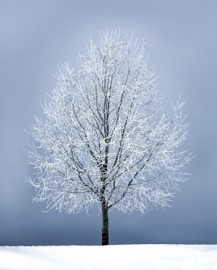
\includegraphics[width=0.7\textwidth]{pics/real_tree.jpg}
	        \tiny{https://images.pexels.com/photos/3732527/pexels-photo-3732527.jpeg}
		\end{figure}
	\end{columns}
\end{frame}

\begin{frame}
	\frametitle{How do Decision Trees Work?}
	\begin{columns}[onlytextwidth]
		\column{0.4\textwidth}
		\begin{block}{Algorithm}
			\begin{enumerate}
				\item Split: find best ``yes/no'' question on best feature		
				\item Apply Step 1 recursively
			\end{enumerate}
		\end{block}
	
		\begin{exampleblock}{Notes}
			\begin{itemize}
				\item ``best'' regarding average loss improvement
				\item Typical losses: squared error, 
				
				log loss/cross-entropy/ 
				
				information or Gini
				\item Predictions?
			\end{itemize}
		\end{exampleblock}
	
		\begin{example}
		\end{example}
	
		\column{0.6\textwidth}
		\begin{figure}
			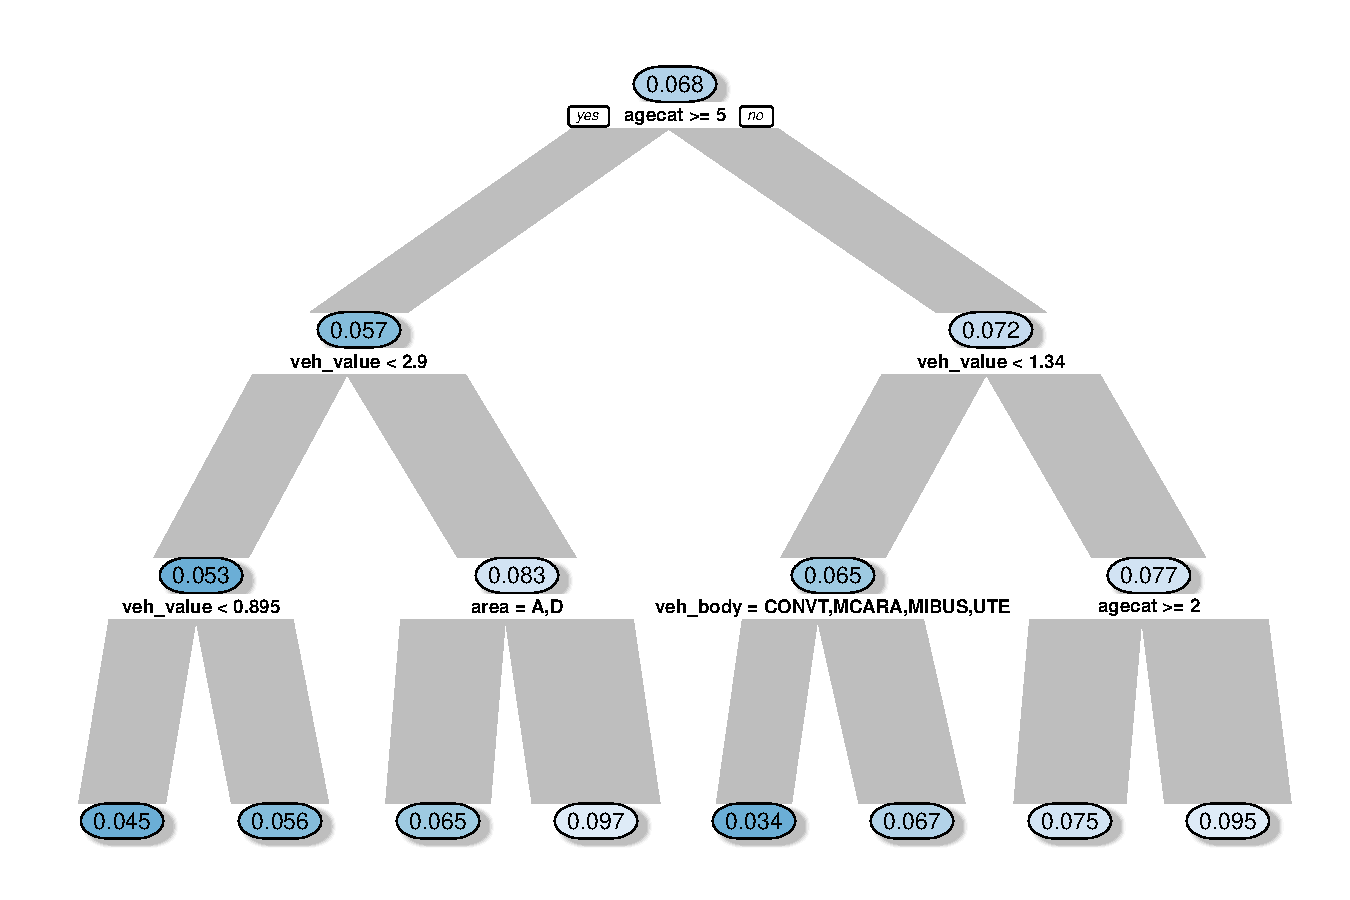
\includegraphics[width=1\textwidth]{pics/tree.pdf}
		\end{figure}
		\centering The tree does a headstand
	\end{columns}
\end{frame}

\begin{frame}
	\frametitle{Properties of Decision Trees}
	\begin{figure}
		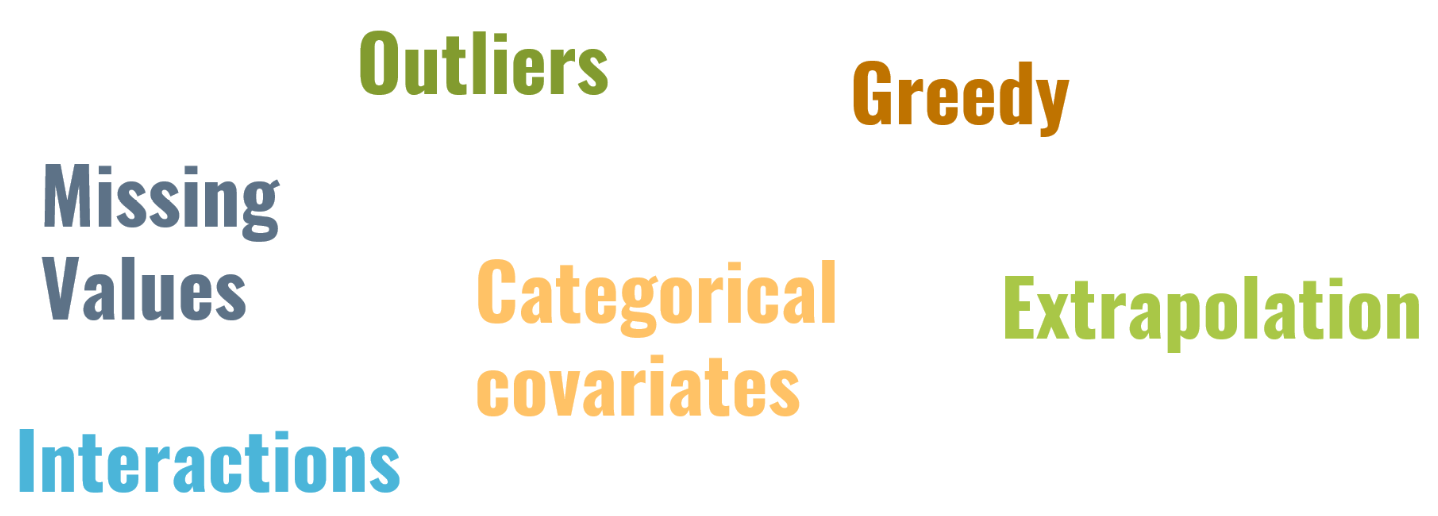
\includegraphics[width=0.7\textwidth]{pics/tree_words.png}
	\end{figure}
	
	\vfill
	
	\centering Properties are inherited to groups/ensembles of decision trees
\end{frame}

%=====================================================================
\subsection{Random Forests}
%=====================================================================

\begin{frame}
	\frametitle{Random Forests}
	\begin{columns}[onlytextwidth]
		\column{0.5\textwidth}
		\begin{itemize}
			\item Combine many decision trees
			\item Perform very well
			\item Black Box
			\item Around since 2001 (Breiman)
		\end{itemize}
		
		\column{0.5\textwidth}
		\begin{figure}
			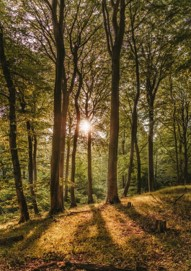
\includegraphics[width=0.6\textwidth]{pics/real_forest.jpg}
			\tiny{https://images.pexels.com/photos/1459534/pexels-photo-1459534.jpeg}
		\end{figure}
	\end{columns}
\end{frame}

\begin{frame}
	\frametitle{How do Random Forests Work?}
	If we train 500 trees, how can we make sure they are different? 
	
	\vfill
	
	\begin{block}{Idea: Introduce two sources of randomness}
		\begin{enumerate}
			\item Each tree is trained on bootstrap sample.
			\item Each split considers random selection of features only.
		\end{enumerate}
	\end{block}

	\vfill

	Predictions? 
\end{frame}

\begin{frame}
	\frametitle{Comments on Random Forests}
	\begin{figure}
		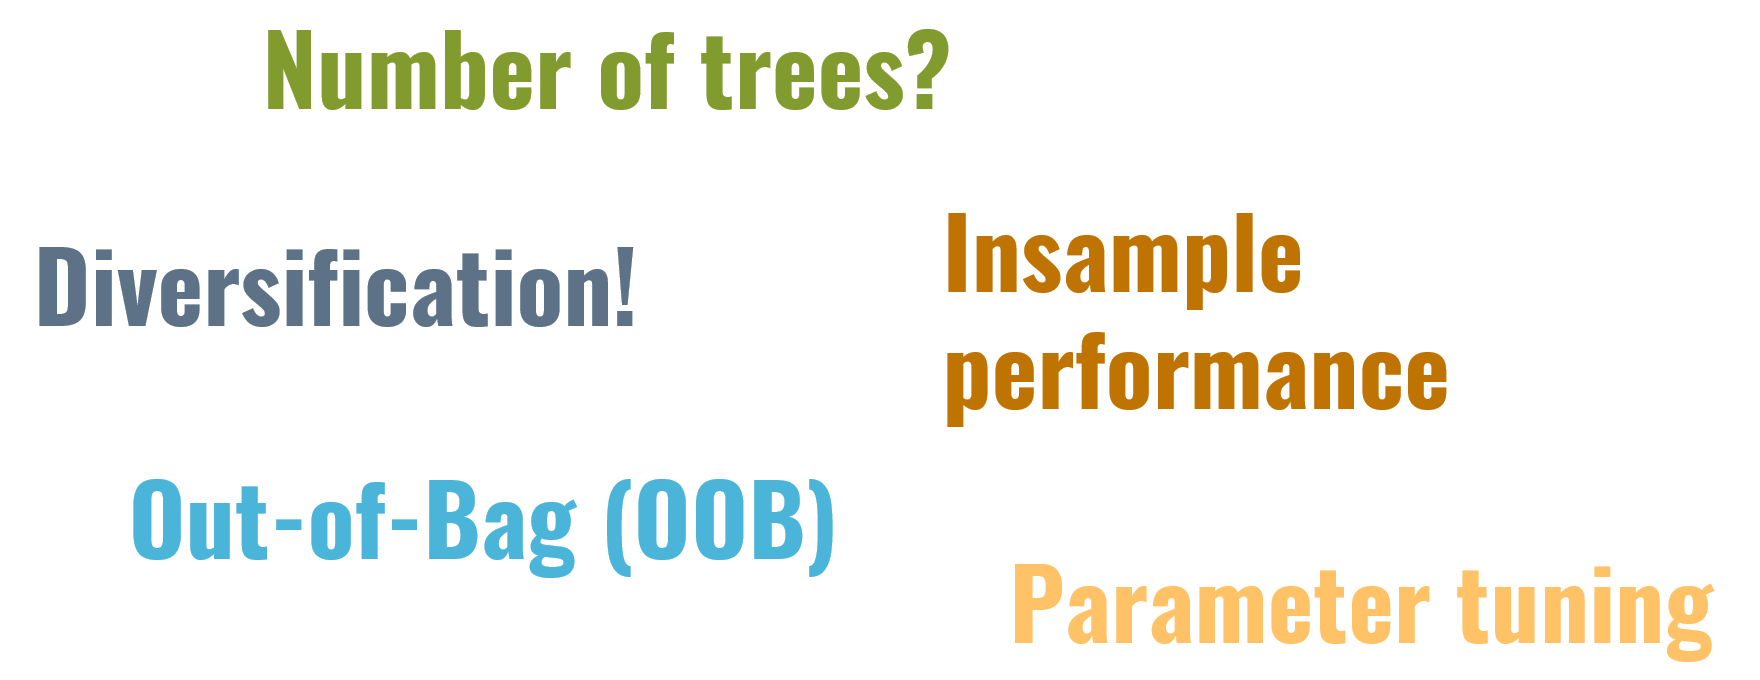
\includegraphics[width=0.8\textwidth]{pics/rf_words.png}
	\end{figure}
	\begin{example}
	\end{example}
\end{frame}

\begin{frame}
	\frametitle{Interpreting a Black Box is Important}
	\begin{block}{Minimum interpretation of model?}
		\begin{enumerate}
			\item Performance
			\item Variable importance
			\item Effects $\rightarrow$ e.g. partial dependence plots
		\end{enumerate}
	\end{block}

	\vfill
	
	\begin{example}
	\end{example}
\end{frame}

\begin{frame}
	\frametitle{Exercises on Random Forests}
	\begin{enumerate}
		\item In our diamonds random forest, replace carat by log(carat). Do the results change?
		
		\vfill
		
		\item Fit a (probability) random forest on the claims data to predict claim probability by {\ttfamily veh\_value}, {\ttfamily veh\_body}, {\ttfamily veh\_age}, {\ttfamily gender}, {\ttfamily area}, and {\ttfamily agecat}.
		\begin{itemize}
			\item Choose tree depth by OOB performance or CV.
			\item Evaluate the model on an independent test dataset.
			\item Interpret the results.
		\end{itemize}
	\end{enumerate}
\end{frame}

%=====================================================================
\subsection{Gradient Boosted Trees}
%=====================================================================

\begin{frame}
	\frametitle{Gradient Boosted Trees}
	\begin{columns}[onlytextwidth]
		\column{0.5\textwidth}
		\begin{itemize}
			\item Combine many decision trees
			\item Perform very well
			\item Black Box
			\item Around since 2001 (Friedman)
			\smash{\raisebox{.6\dimexpr3\baselineskip+0\itemsep+5\parskip}{$\left.\rule{0pt}{.6\dimexpr4\baselineskip+0\itemsep+6\parskip}\right\}\text{\rotatebox[origin=c]{90}{\footnotesize \alert{Like random forests}}}$}}
			\item \href{https://github.com/mayer79/gradient_boosting_comparison}{XGBoost, LightGBM, CatBoost}
		\end{itemize}
		
		\column{0.5\textwidth}
		\begin{figure}
			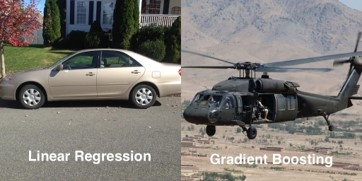
\includegraphics[width=0.95\textwidth]{pics/helicopter.jpg}
			\tiny{https://www.gormanalysis.com/blog/gradient-boosting-explained/}
		\end{figure}
	\end{columns}
\end{frame}

\begin{frame}
	\frametitle{How does Gradient Boosting Work?}
	\begin{columns}[onlytextwidth]
		\column{0.55\textwidth}
		\begin{block}{Algorithm}
			\begin{enumerate}
				\item Fit simple model 
				
				(often a small decision tree).
				\item Add another simple model to 
				
				correct errors of first model.
				\item Repeat Step 2 until stopping
				
				criterion triggers.
			\end{enumerate}
		\end{block}
		\column{0.45\textwidth}
		\begin{alertblock}{Remarks}
			\begin{itemize}
				\item Completely different from 
				
				random forest.
				\item Predictions are found by combining predictions of all simple models (like random forest).
				\item Flexible regarding loss function.
			\end{itemize}
		\end{alertblock}
	\end{columns}

	\vfill

	\begin{exampleblock}{\centering Example XGBoost}
	\end{exampleblock}
\end{frame}

\begin{frame}
	\frametitle{Parameter Tuning is Essential}
	\begin{columns}[onlytextwidth]
		\column{0.7\textwidth}
		\begin{enumerate}
			\item Number of boosting rounds/trees 
			
			$\rightarrow$ find by early stopping (validation/CV)
			\item Learning rate 
			
			$\rightarrow$ to get reasonable number of rounds
			\item Regularization
				\begin{itemize}
					\item Tree depth, number of leaves, loss penalties, etc.
					\item $\rightarrow$ Grid/Randomized search and iterate
				\end{itemize}
		\end{enumerate}
		\column{0.3\textwidth}
		\begin{alertblock}{Why not one big 
				
				grid search on 
				
				all parameters?}
		\end{alertblock}
	\end{columns}

	\vfill
	
	\begin{exampleblock}{\centering Example XGBoost}
	\end{exampleblock}
\end{frame}

\begin{frame}
	\frametitle{Exercises on Gradient Boosting}
	\begin{enumerate}
		\item Study online documentation of XGBoost to make the last model monotonically increasing in carat. Check the resulting partial dependence plot.
		
		\vfill
		
		\item Develop a strong XGBoost model on the claims data to predict claim probability by {\ttfamily veh\_value}, {\ttfamily veh\_body}, {\ttfamily veh\_age}, {\ttfamily gender}, {\ttfamily area}, and {\ttfamily agecat}.
		\begin{itemize}
			\item Use \alert{{\ttfamily ``binary:logistic''}} as objective.
			\item Use \alert{{\ttfamily ``logloss''}} as evaluation metric.
			\item Use a clean CV/test strategy.
			\item Interpret the results.
		\end{itemize}
	\end{enumerate}
\end{frame}

%=====================================================================
\section{Neural Nets}
%=====================================================================

\begin{frame}
	\frametitle{Neural Nets}
	\begin{itemize}
		\item Around since the 1950ies
		\item Underwent different development steps, e.g.
		\begin{itemize}
			\item use of backpropagation
			\item GPUs
		\end{itemize}
		\item Black Box
		\item TensorFlow/Keras, PyTorch
	\end{itemize}
\end{frame}

\begin{frame}
	\frametitle{``Swiss Army Knife'' among ML Algorithms}
	\begin{figure}
		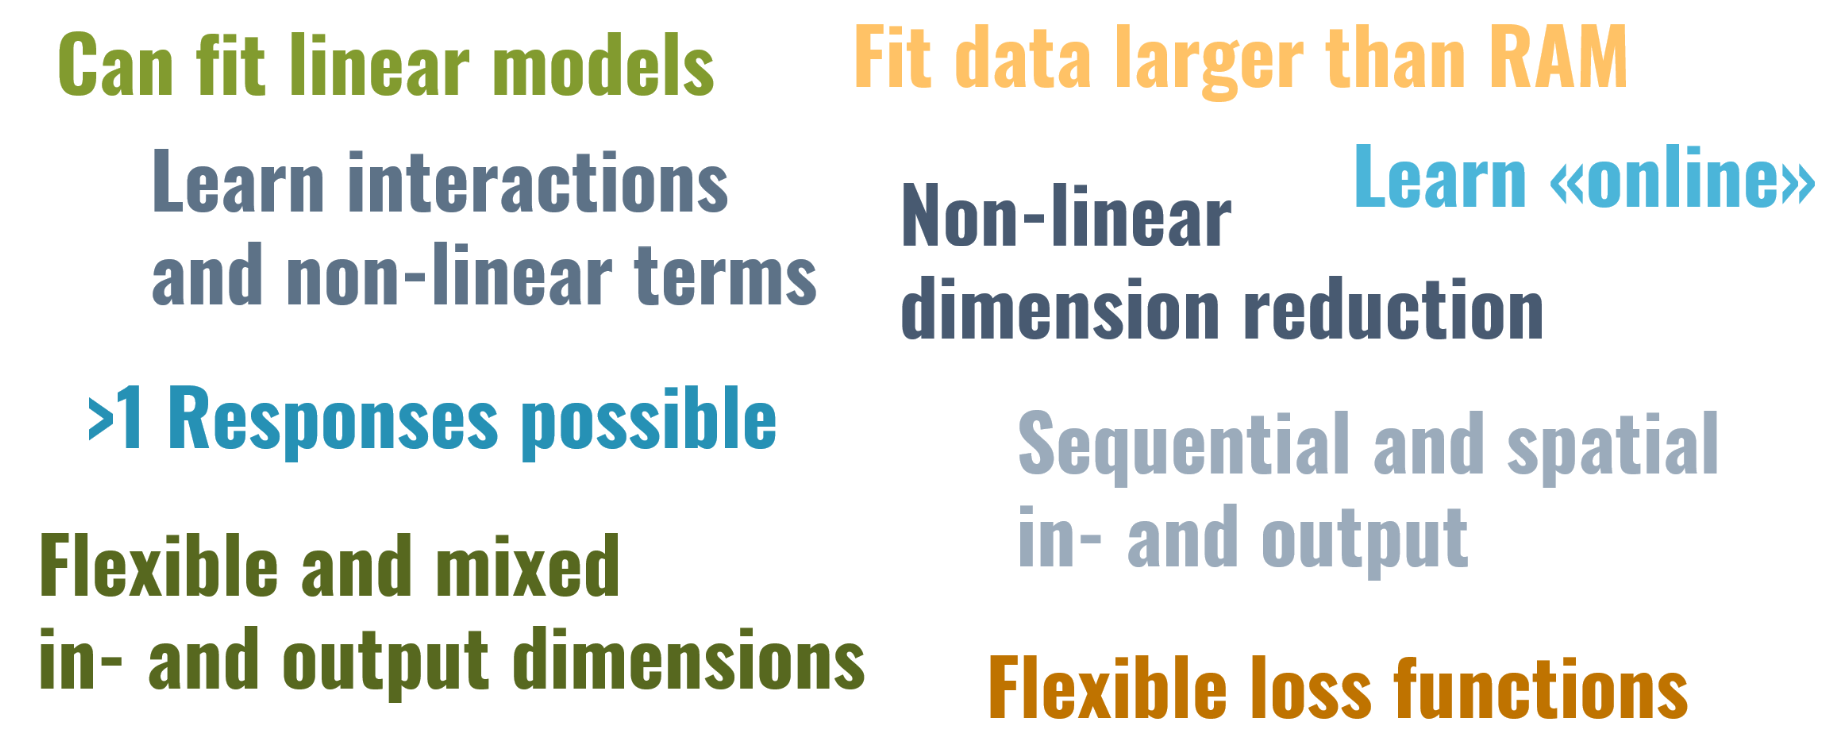
\includegraphics[width=0.9\textwidth]{pics/nn_knife.png}
	\end{figure}
\end{frame}

\begin{frame}
	\frametitle{Understanding Neural Nets in three Steps}
	\begin{enumerate}
		\item Linear regression as neural net
		\item Hidden layers
		\item Activation functions
	\end{enumerate}

	\vfill
	
	Using \alert{diamonds} data
\end{frame}

\begin{frame}
	\frametitle{Step 1: Linear Regression as Neural Net}
	\begin{columns}
		\column{0.35\textwidth}
		\begin{itemize}
			\item $E(\text{price})=\alpha+\beta \cdot \text{carat}$
			\item OLS 
			
			$\hat\alpha \approx -2256$, $\hat\beta \approx 7756$
			\item Represented as neural network graph
		\end{itemize}
		\column{0.65\textwidth}
		\begin{figure}
		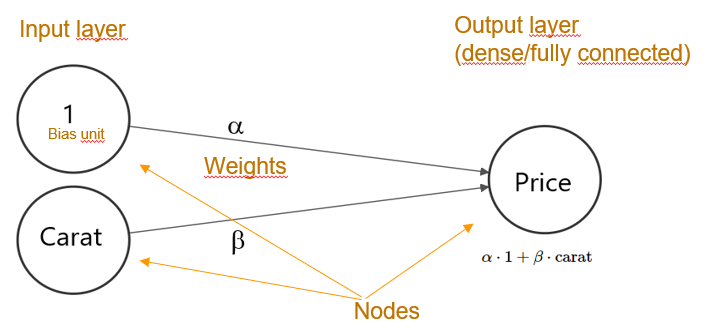
\includegraphics[width=0.9\textwidth]{pics/simple_nn.png}
	\end{figure}
	\end{columns}
	
	\vfill

	\begin{exampleblock}{\centering Example}
	\end{exampleblock}
\end{frame}

\begin{frame}
	\frametitle{The Optimization Algorithm}
	\begin{block}{``Mini-batch gradient descent with \alert{backpropagation}''}
		\begin{enumerate}
			\item Init step: Randomly initiate parameters.
			\item Forward step: Use parameters to calculate predictions of \alert{batch}.
			\item Backprop step: Evaluate \alert{average loss} (e.g. MSE) of batch. Change parameters systematically to make it smaller.
			\item Repeat Steps 2 and 3 until one \alert{epoch} is over.
			\item Repeat Step 4 until some stopping criterion triggers.
		\end{enumerate}
	\end{block}

	\vfill

	SGD? Gradients? Local minima?
\end{frame}

\begin{frame}
	\frametitle{Step 2: Hidden Layers}
	\begin{columns}
		\column{0.33\textwidth}
		\begin{itemize}
			\item Add \alert{hidden layers} for more parameters 
			
			(= flexibility)
			\item Their nodes are latent/implicit variables
			\item Representational learning
			\item \small{\alert{Encoding}?}
			\item \small{\alert{Deep} neural net?}
		\end{itemize}
		\begin{example}
		\end{example}
		\column{0.67\textwidth}
		\begin{figure}
			\includegraphics[width=0.98\textwidth]{../figs/nn_1_hidden.png}
		\end{figure}
	\end{columns}
\end{frame}

\begin{frame}
	\frametitle{Step 3: Activation Functions}
	Non-linear transformations $\sigma$ of node values necessary!
	\begin{columns}[onlytextwidth]
		\column{0.35\textwidth}
		\begin{itemize}
			\item tanh: $\sigma(x) = \frac{e^x - e^{-x}}{e^x + e^{-x}}$
			\item ReLU: $\sigma(x) = \text{max}(0, x)$
		\end{itemize}
		\begin{figure}
			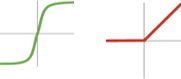
\includegraphics[width=0.8\textwidth]{pics/activation_functions.png}
		\end{figure}
		\begin{block}{Two purposes}
			\begin{itemize}
				\item Imply interactions and non-linear terms
				\item Inverse link as in GLMs
			\end{itemize}
		\end{block}
		\begin{example}
		\end{example}
		\column{0.65\textwidth}
		\begin{figure}
			\includegraphics[width=0.98\textwidth]{../figs/nn_activation.png}
		\end{figure}
	\end{columns}
\end{frame}

\begin{frame}
	\frametitle{Practical Considerations}
	\begin{figure}
		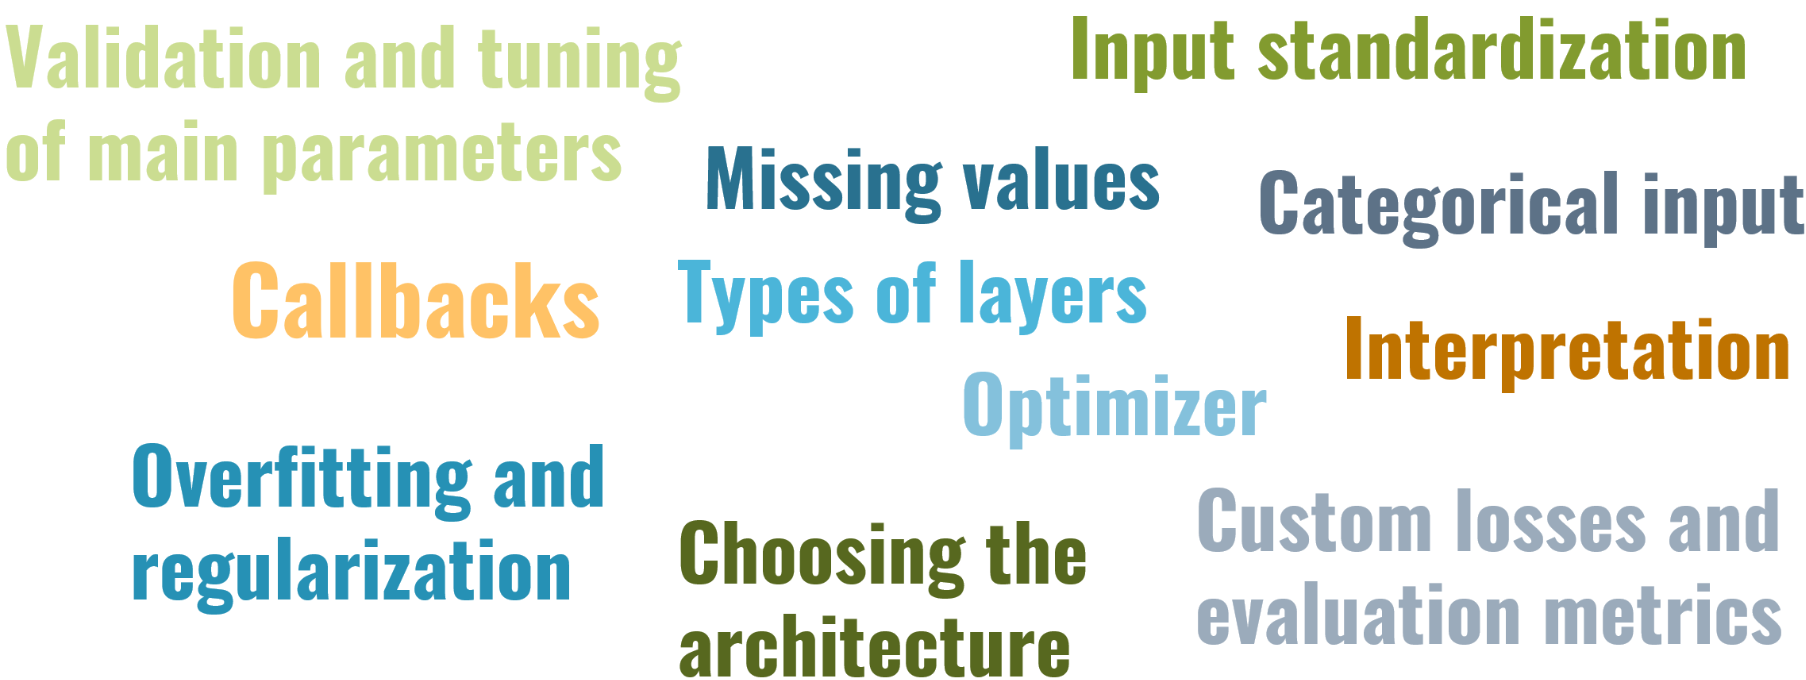
\includegraphics[width=0.9\textwidth]{pics/nn_practical.png}
	\end{figure}
\end{frame}

\begin{frame}
	\frametitle{Example: diamonds}
	\begin{figure}
		\includegraphics[width=0.6\textheight]{../figs/nn_2_hidden.png}
	\end{figure}
\end{frame}

\begin{frame}
	\frametitle{Exercises on Neural Nets}
	\begin{enumerate}
		\item Fit diamond prices by minimizing Gamma deviance with log-link 
		
		(custom loss as in lecture notes; log-link means "exponential" output activation)
		\begin{itemize}
			\item Tune model by simple validation.
			\item Evaluate final model (for simplicity) on validation data.
			\item Interpret final model.
		\end{itemize}
		Hints: Use smaller learning rate and replace ``relu'' by ``tanh''. Furthermore, the response is to be transformed from int to float.
		
		\vfill
		
		\item Study either the optional claims data example in the lecture notes or build your own neural net, predicting claim yes/no.
	\end{enumerate}
\end{frame}

%=====================================================================
\section{Final Words}
%=====================================================================

\begin{frame}
	\frametitle{Comparison of ML Algorithms}
		\begin{figure}
		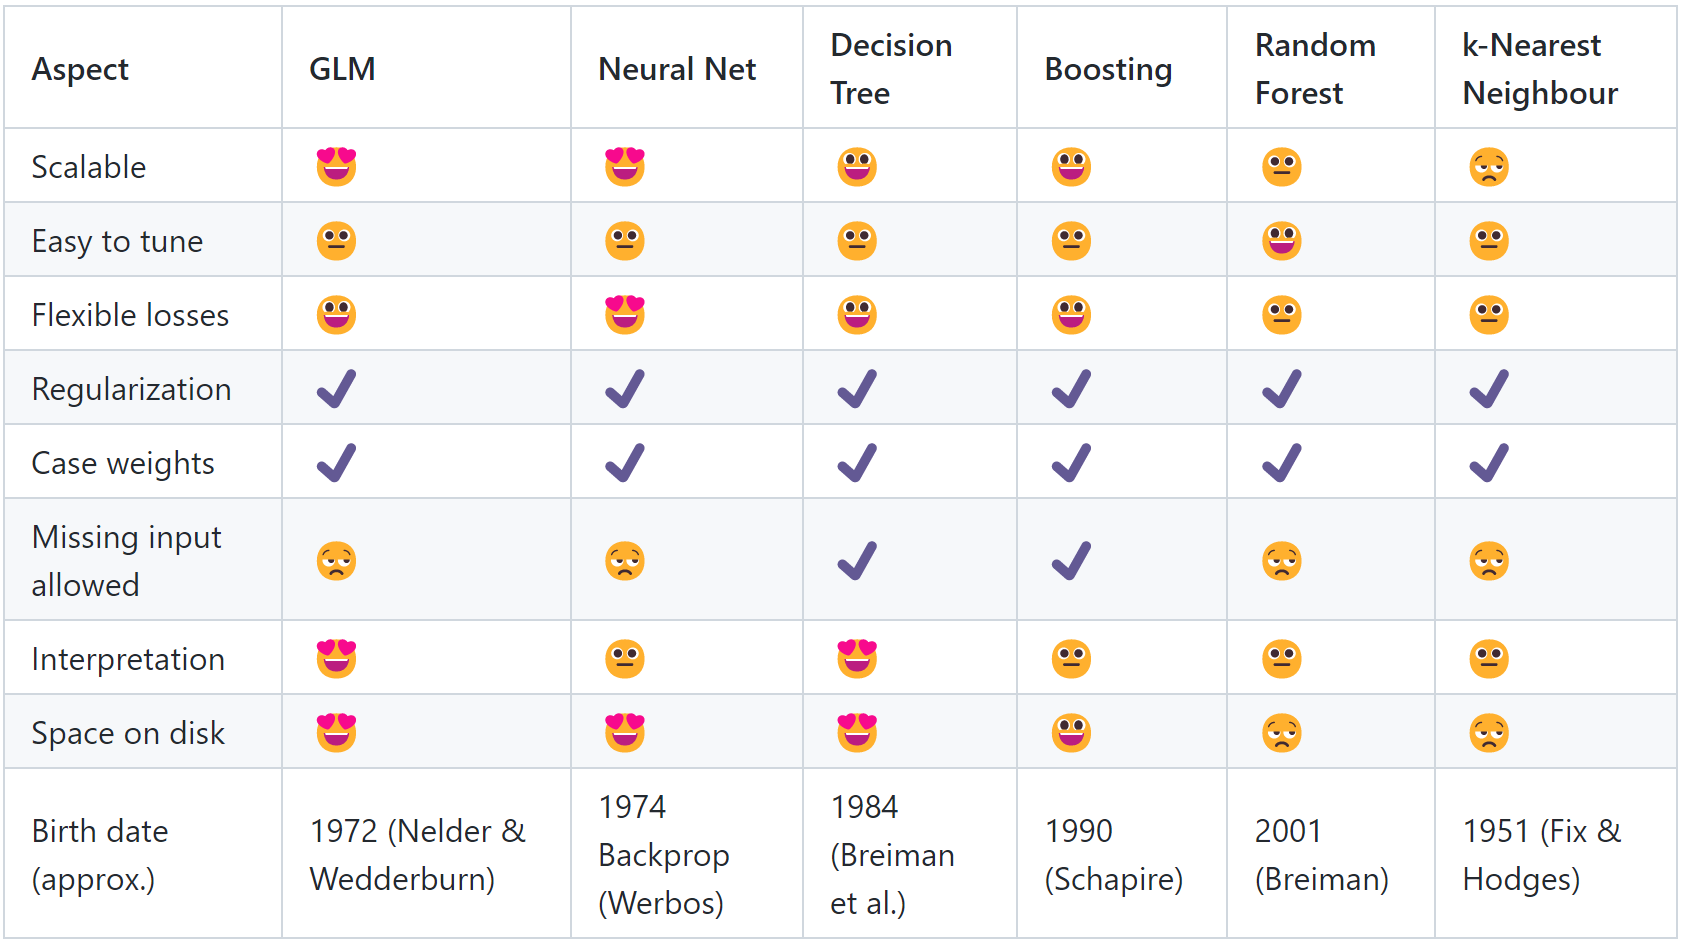
\includegraphics[width=0.9\textwidth]{pics/algorithms.png}
	\end{figure}
\end{frame}

\begin{frame}
	\frametitle{``Michael’s Analysis Scheme X''}
	\begin{enumerate}
		\item Take any property $T(Y)$ of key interest (churn rate, claims frequency, loss ratio, etc.) and calculate its value on the full dataset.
		\item Do a descriptive analysis of $T(Y \mid X_j)$ for a couple of covariates to study the bivariate association between $Y$ and each $X_j$ separately.
		\item Accompany Step 2 by ML model $T(Y\mid X_1, \dots, X_p) \approx f(X_1, \dots, X_p)$
			\begin{itemize}
				\item Check its performance.
				\item Study variable importance and use it to sort the results of Step 2.
				\item Study partial (or SHAP) dependence plots for each $X_j$ and compare them with the associations from Step 2.
			\end{itemize}
	\end{enumerate}

	\vfill
	
	\begin{block}{What did you learn from Step 3?}
	\end{block}
\end{frame}

%=====================================================================
\end{document}
%=====================================================================